\documentclass[12pt,a4paper]{article}
\usepackage[utf8]{inputenc}
\usepackage{amsmath}
\usepackage{amsfonts}
\usepackage{amssymb}

%bold Greek letters and other symbols
\usepackage{bm}

\usepackage[T1]{fontenc}
\usepackage[english]{babel}
\usepackage{graphicx}
\usepackage[left=2.5cm,right=2.5cm,top=2.5cm,bottom=2cm]{geometry}
\usepackage{color}
%
\usepackage{makeidx}
\usepackage{shortvrb,latexsym}

\setlength{\parindent}{0pt}
%\renewcommand{\floatpagefraction}{.99}
%\renewcommand{\textfraction}{.01}

\newcommand{\bu}{{\bf u}}
\newcommand{\bv}{{\bf u}}
\newcommand{\rd}{\mathrm{d}}
\newcommand{\hx}{{\bf\hat{x}}}
\newcommand{\hy}{{\bf\hat{y}}}
\newcommand{\hz}{{\bf\hat{z}}}
\newcommand{\hr}{{\bf\hat{r}}}
\newcommand{\hn}{{\bf\hat{n}}}

\begin{document}

\begin{center}
2019-01-16
\end{center}
STOCKHOLMS UNIVERSITET\\
Meteorologiska Institutionen\\
Jonas Nycander, Dhrubaditra Mitra\\
\vspace{1cm}

\begin{center}
{\bf\large Exam in Fluid mechanics (MO5001)}\\
\end{center}

Write the solution of each problem on a separate paper, and write your identification number on every paper.\\

{\bf Allowed aids:} calculator, sheet with vector analysis relations.\\

{\bf Grading:} A 90-100\%, B 80-89\%, C 65-79\%, D 55-64\%, E 50-54\%, Fx 45-49\%, F 0-44\% \\
\vspace{0.5cm}

\begin{enumerate}
%====================================================================
\item {\bf Egyptian water clock:}
  An Egyptian water clock, is a bowl with a small hole at the
  bottom. Time is measured by the fall of water level in this bowl as
  water flows out of the small hole in the bottom. To be able to
  function as a clock the rate of fall of the water level must be
  constant as a function of time for some interval of time.
  Wikipedia states: ``The oldest documentation of the water clock is
  the tomb  inscription
  of the 16th century BC Egyptian court official Amenemhet,
  which identifies himself as its inventor''. Let us see if you can
  design one.   The bowl is a surface of revolution whose
  cross-section is shown in figure~\ref{fig:clock}.
  The surface is well-defined if we give the radius of the bowl, $R(H)$
  as a function of its height $H$.
  \begin{figure}[h]
    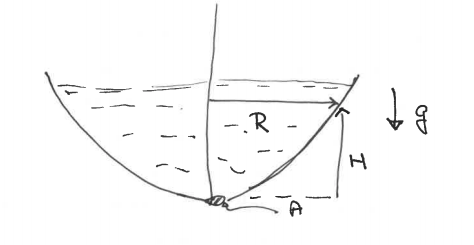
\includegraphics[width=0.5\linewidth]{egypt.png}
    \label{fig:clock}
   \end{figure}
  \begin{enumerate}
\item At time $t$, let the height of the water in the bowl be
  $H(t)$. What is the velocity, $v(t)$, of the water flowing out of the hole at
  that instant ?  Write clearly what assumptions you have made in
  arriving at the answer.
  \item If the area of the hole is $A$, the rate at which water flows
    out of the hole $Q = v A C $ where $C$ is an emperically
    determined constant. In a small time $\Delta t$, the amount of
    water that flows out of this hole is give by $Q\Delta t$. If the
    fall in height in this small interval of time is $\Delta H$ then
    \begin{equation}
      Q\Delta t = \pi R^2(H)\Delta H
      \end{equation}
    where $R$ is the radius of the bowl at the height $H$. To be able
    to function as a clock the rate of fall of $H$ must be a
    constant. Find $H$ as a function of $R$.
  \item If an ancient egyptian brought this clock from Egypt to Sweden
    will it work equally well ? 
  \end{enumerate}

(12 p) \\


  \item While cooking last night, I put my chopping board on the
    kitchen counter. I had not noticed that there was a small amount
    of water on the kitchen counter already. After using the board I
    tried to lift it up in the way I sketch in
    figure~\ref{fig:board}. I realised that I had to exert a force much
    larger than the weight of the board itself.
  \begin{figure}[h]
    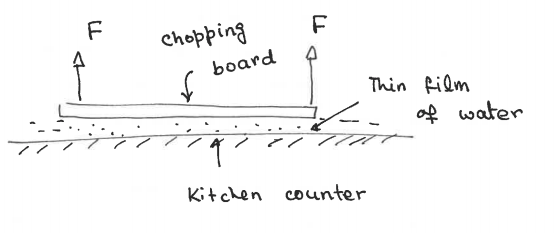
\includegraphics[width=0.5\linewidth]{board.png}
    \label{fig:board}
   \end{figure}
    \begin{enumerate}
    \item Explain qualitatively (and concisely) why ?
    \item Assume that the shape of my chopping board is a circular
      disk of radius $a$. The thickness of the film of
      water trapped between the board and the kitchen counter is $h$.
      Calculate the force necessary to pull the board by a distance
      $\Delta h$ in time $\Delta t$. State clearly all the assumption
      you need to make to solve this problem.
    \end{enumerate}

(13 p)\\


  \item 
The horizontal component of the Navier-Stokes equations in a rotating 
system is
$$
\frac{\partial\bu}{\partial t}+\bu\cdot\nabla\bu+f\hz\times\bu = 
-\frac{\nabla p}{\rho}+\nu\nabla^2 \bu,
$$
where the velocity $\bu$ is assumed to be purely horizontal.

a) Define the Rossby number and the Ekman number in terms of the time
scale $T$, horizontal length scale $L$ and vertical length scale $H$.
Also give the thickness of the Ekman layer.

b) Simplify the equation above for the case that $\bu$ is stationary
and horizontally homogeneous, i.e.\ does not depend on $t, x$ or $y$.

c) A constant wind blows over the ocean and exerts the wind stress
$\bm{\tau}$ on the surface of the ocean. Give the appropriate 
boundary condition for the flow $\bu$ in the ocean.

d) Assume that there is no geostrophic flow, and determine the mass 
flux in the ocean Ekman layer.

(10 p)\\
%====================================================================
\item
The rotating and linearized shallow-water equations are solved with the 
initial conditions
$$
\bu=0
$$
$$
\eta = \left\{
\begin{array}{rcl}
\eta_0, \quad x <  0 \\
-\eta_0, \quad x  > 0 \\
\end{array}
\right.
$$
where $\bu$ is the velocity and $\eta$ the surface perturbation. The 
Coriolis parameter $f$ is constant. What determines the asymptotic state
as $t\rightarrow\infty$? Describe qualitatively the asymptotic state and 
the evolution toward it, sketching $\bu$ and $\eta$.

(5 p)\\
%====================================================================
\item 
The rotating shallow-water equations are
$$
\frac{\partial \bu}{\partial t}+\bu\cdot\nabla\bu+f\hz\times\bu
= -g\nabla\eta,
$$
$$
\frac{\partial h}{\partial t}+\nabla\cdot[\bu(H+\eta)] = 0,
$$
where $H$ is the mean depth and $\eta$ the surface  perturbation.

a) What assumptions are made in order to derive the quasigeostrophic
vorticity equation from the equations above?

b) What is the most important difference between the rotating shallow-water
equations and the quasigeostrophic vorticity equation regarding the 
phenomena that these two models can describe? What assumption leads
to this difference, and why?

c) Derive the quasigeostrophic potential vorticity from the potential  
vorticity that is exactly conserved by the rotating shallow-water 
equations.

(10 p)\\
%====================================================================
\end{enumerate}
\end{document}
